\documentclass{article}
\usepackage{graphicx} 
\usepackage{float}
\title{Platformio Question}
\author{GALI SAI AJAY}
\date{\today}

\begin{document}

\maketitle

 For the $3$-bit binary counter shown in the figure, the output increments at every positive 
transition in the clock (CLK). Assume ideal diodes and the starting state of the counter as 
$000$. If output high is $1 V$ and output low is $0 V$, the current $I$(in mA) flowing through the 
$50 \Omega$ resistor during the $5$th clock cycle is (up to one decimal place)
\begin{figure}[H]
\centering
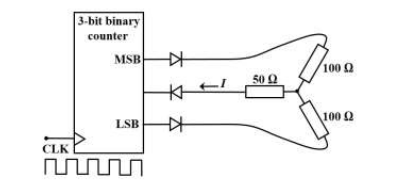
\includegraphics[width=\columnwidth]{pic.png}
\caption{circuit}
\label{fig:lcd}
\end{figure}

\end{document}
